\documentclass[12pt]{report}
\usepackage[a4paper,left=30mm,right=25mm,top=25mm,bottom=25mm]{geometry}
\usepackage[utf8]{inputenc}
\usepackage[english,hungarian]{babel}
\usepackage{t1enc}
\usepackage{graphicx}
\usepackage{caption}
\usepackage{marginnote}
\usepackage{listings}
\usepackage{color}
\usepackage{newtxtext,newtxmath} % times new roman imitation
\usepackage{graphicx}
\usepackage{setspace}
\usepackage{tabularx}
\usepackage{mathtools}
\usepackage{float}
\usepackage{fancyhdr}
\usepackage{makeidx} % indexing enable
\graphicspath{ {images/} }
\usepackage{emptypage}

\newcommand\blankpage{%
    \null
    \thispagestyle{empty}%
    \addtocounter{page}{-1}%
    \newpage}

\usepackage[totoc]{idxlayout}

\linespread{1.5}

\makeindex

% Equation capture settings
\DeclareCaptionType{equ}[][List of equations]
\captionsetup[equ]{labelformat=empty}

% Figure caption settings
\renewcommand{\thefigure}{\arabic{chapter}-\arabic{figure}}

% Table caption settings
\renewcommand{\thetable}{\arabic{chapter}-\arabic{table}}

% Code listing styles
\definecolor{codegreen}{rgb}{0,0.6,0}
\definecolor{codegray}{rgb}{0.5,0.5,0.5}
\definecolor{codepurple}{rgb}{0.58,0,0.82}
\definecolor{backcolour}{rgb}{0.95,0.95,0.92}

\lstdefinestyle{codestyle}{
    backgroundcolor=\color{backcolour},   
    commentstyle=\color{codegreen},
    keywordstyle=\color{magenta},
    numberstyle=\tiny\color{codegray},
    stringstyle=\color{codepurple},
    basicstyle=\ttfamily\footnotesize,
    breakatwhitespace=false,         
    breaklines=true,                 
    captionpos=b,                    
    keepspaces=true,                 
    numbers=left,                    
    numbersep=5pt,                  
    showspaces=false,                
    showstringspaces=false,
    showtabs=false,                  
    tabsize=2
}
\lstset{style=codestyle}

\usepackage[bibstyle=authoryear,
            citestyle=authoryear,
            backend=biber,
            sorting=nyt]{biblatex}
\addbibresource{bibliography.bib}

\usepackage{hyperref}

\renewcommand{\labelenumii}{\roman{enumii})} % list: second level is roman numerals

\title{
RELNORM: RELÁCIÓS ADATBÁZISOK NORMALIZÁLÁSÁHOZ HASZNÁLT ESZKÖZ AZ OKTATÁSBAN
}

\author{Kiss Gergely}
\date{Temesvár, 2022}

\begin{document}

\makeatletter
\renewcommand\maketitle{
{
\begin{center}

\includegraphics{logo} \\[4ex]
\Large \uppercase{Tudományos diákköri dolgozat}
\end{center}
%\raggedright % Note the extra {
\vspace{1cm}
\begin{center}
{\Huge \bfseries \uppercase{\@title} }\\
\vspace{2cm}
\newcolumntype{R}{>{\raggedleft\arraybackslash}X}%
\centering
\large{
\begin{tabularx}{\textwidth}{R X}
\textbf{Szerző:} &  \textbf{\@author} \\
         & Számítástechnika MSc. szak, I. évf. \\[4ex]
\textbf{Konzulens:} & \textbf{Milan Čeliković} \\
& egyetemi docens
\end{tabularx}
}
\end{center}}
} % Note the extra }

\begin{titlepage}
\thispagestyle{fancy}
\fancyhf{}
\renewcommand{\headrulewidth}{0pt}
\cfoot{Temesvár, 2022}
\maketitle
\end{titlepage}

\blankpage
\newpage
\pagenumbering{gobble}
\linespread{1}

\begin{center}
    {\bfseries
    \vspace*{1.5cm}
    \large{SAPIENTIA ERDÉLYI MAGYAR TUDOMÁNYEGYETEM} \\\vspace{2.5cm}
    \large{\@title} \\ \vspace{1.5cm}
    \large{RELNORM: RELATIONAL DATABASE NORMALIZATION TOOL IN EDUCATION} \\ \vspace{2cm}
    }
    \large{
    \@author \\ \vspace{2cm}
    
    Konzulens: \\
    Milan Čeliković
    \vfill
    Kézirat lezárva: 2022. április 11.
    }
\end{center}
\blankpage
\blankpage
\selectlanguage{english}
\begin{abstract}
    
The use of relational databases and database normalization problems have been a field of interest to many computer scientists over the decades. There have been many solutions to these problems over the years, but there are still gaps in some aspects. As a teaching assistant at the Faculty of Technical Sciences in Novi Sad, we were thinking about developing a program that would be a proper tool for performing teaching assistant tasks. Our main requirement is that the software need to support the normalization algorithms studied at the university: the synthesis and decomposition algorithms. A requirement for the decomposition algorithm is to implement an interactive flow of the algorithm. An additional detail of the requirements was that task series need to be easily specified and replaced.

As a result of these requirements, we developed an application called \textit{RelNorm} to solve the problem of normalizing relational databases as a console application. It is an application written in the \textit{Java} programming language that breaks down a relational schema into multiple relational schemas, depending on the normalization algorithm. Unit tests were used to verify the correctness of the implementation. Code base analysis was done with \textit{SonarCloud} measuring code coverage, reliability and maintainability. The results of the tests and the analysis are included in this paper.

\textit{RelNorm} has already been proven in practice, as it has already been used by teaching assistants in the 2021/2022 academic year to assemble database normalization task series and review solved tasks.

Keywords: relational database, normalization, relational schemas, software testing, code coverage.

\end{abstract}
\blankpage
\selectlanguage{hungarian}
\begin{abstract}

A relációs adatbázisok használata és a velük járó normalizációs problémák már több évtizede foglalkoztatják a számítástechnikában tevékenykedő egyéneket. Az évek során megannyi megoldás született ezekre a problémákra, azok bizonyos aspektusainál mégis hiányosságokat fedezhetünk fel. Az újvidéki Műszaki Tudományok Karán dolgozó tanársegédként egy testreszabott eszköz kifejlesztésében gondolkodtunk, amely kézenfekvő lenne tanársegédi feladatok elvégzéséhez. Fő követelménynek tűztük ki azt, hogy a szoftver támogassa az egyetemen feldolgozott normalizálási algoritmusokat: a szintézis és a dekompozíció algoritmusát. A dekompozíció algoritmusánál további követelmény az algoritmus interaktív lefolyásának a megvalósítása. További részletkövetelmény volt, hogy a feladatsorok könnyen megadhatóak és cserélhetőek legyenek.

Ezen követelmények hatására fejlesztettük ki a \textit{RelNorm} szoftvert, ami a relációs adatbázisok normalizálási problémáját hivatott megoldani konzol applikációként. \textit{Java} programnyelvben íródott applikációról van szó, amely egy relációs sémát bont fel több relációs sémára, a normalizálási algoritmustól függően. Unit-tesztekkel ellenőriztük az algoritmusok helyes megvalósítását, valamint teljes kódbázis elemzést is végrehajtottunk a \textit{SonarCloud} eszközzel. A tesztek eredményét és az elemzést is a dolgozat tartalmazza.

A \textit{RelNorm} a gyakorlatban már bizonyított, ugyanis a 2021--2022-es tanévben már használták a tanársegédek feladatsorok összeállításához és a megoldott feladatlapok átnézésénél.

Kulcsszavak: relációs adatbázis, normalizálás, relációs sémák, szoftvertesztelés, kód lefedettség

\end{abstract}
\blankpage
\selectlanguage{hungarian}
%\addtocontents{toc}{\protect\thispagestyle{empty}}
\pagenumbering{gobble}
\tableofcontents
\listoffigures
\listoftables
%\listofequs
\newpage
\pagenumbering{arabic}
\setcounter{page}{1}

\chapter{Bevezető}

A relációs adatbázisok alapjául szolgáló relációs adatmodell már az 1970-es években sok tudományos munka tárgyát képezte, és az 1990-es évektől kezdve kezdték alkalmazni kommerciális környezetben is \parencite{mogin1996}. Napjainkban a legkülönfélébb vállalkozások is nagy arányban használnak relációs adatbázisokat valamilyen formában, ezt több felmérés [\parencite{scalegrid2019}, \parencite{ramel2015}] és jelentés \parencite{loukides2022} is bizonyítja. Egy nagy előnye a relációs adatbázisoknak, hogy a relációs adatmodell szilárd matematikai alapokra épül. Ezek az alapok többek között a halmazelméletet és a matematikai relációkat foglalják magukban, ami engedélyezi a relációs algebra és kalkulus műveleteinek a használatát \parencite{mogin1996}.

Annak érdekében, hogy egy relációs adatbázison el tudjunk végezni bizonyos relációs műveleteket, és pontos eredményekhez jussunk, elengedhetetlen az a feltétel, hogy az adatainkat veszteségmentesen egyesíthető relációkba szervezzük. Veszteséges egyesítésnél adatok tűnhetnek el, vagy megjelenhetnek további téves adatok. Ezen probléma kiküszöböléséhez adatbázis normalizálást kell végrehajtanunk, amivel a relációs sémákat átszervezzük olyan formába, amely veszteségmentes egyesítést eredményez. Ezen normalizálási műveletek sikeres elvégzéséhez a dolgozat két algoritmust is bemutat.

Jelenleg az Újvidéki Egyetem munkatársa vagyok, a Műszaki Tudományok Karán végzek tanársegédi feladatokat. Ezen a karon több szakirányon is folyik relációs adatbázistervezéssel foglalkozó tárgy. A tárgy neve Adatbázisok 2 \parencite{ftn2021}, melynek keretén belül előadjuk az említett normalizálási algoritmusokat is. Az algoritmusokat feladatok kíséretében dolgozzuk fel kézileg és ugyanígy papíron történik a hallgatók vizsgáztatása is. Egy feladatlap elkészítése, megoldáskulcs ellenőrzése, majd a későbbi hallgatók által kitöltött feladatlapok átnézése potenciálisan sok időt felemészt, valamint nagy felelőséggel is jár. A dekompozíció normalizálási algoritmusa választási lehetőség elé állítja az alanyt, vagyis különböző útvonalakon juthat el a hallgató a helyes eredményig. Ez az interaktív mozzanat tovább bonyolítja a megoldott feladatok kiértékelését – adott esetben a részeredmények helyességének a megállapítását.

Annak érdekében, hogy enyhítsünk a tanársegédekre helyezedő nehézségeken, kifejlesztettük a \textit{RelNorm} nevezetű szoftvert, mely képes pontosan elvégezni a relációs adatbázis normalizálási feladatait, lehetővé téve az interaktív lépések végrehajtását. A szoftver emellett még megkönnyíti a feladatsorok megadási módját is, ezzel is felgyorsítja a feladatok kidolgozásának a folyamatát.

A bevezető mondatok után először egy irodalmi áttekintés következik, majd a dolgozat célkitűzéseit definiáljuk. Az ezt követő fejezeteket a szoftver kifejlesztésének elméleti háttere, relációs alapfogalmak és algoritmusok bemutatása követi. A bemutatott algoritmusok megvalósításáról lesz szó az ezt követő fejezetben, majd későbbi fejezetekben a szoftvertesztelés és annak eredményeinek az elemzése kap helyet. Végül záró fejezetként összefoglalásra kerülnek a dolgozatban leírtak.

\chapter{Irodalom áttekintés}

A bevezető részben már szó volt a relációs adatmodell történetéről, és arról a tényről is, hogy már a múlt század második felében sok kutatói munka tárgyát képezte. Átfogó és bizonyított elméleti alapokkal vághatunk tehát neki a téma kidolgozásának. Ebben a dolgozatban az újvidéki Műszaki Tudományok Karán is tekintélyes irodalomra támaszkodunk \parencite{mogin1996}, \parencite{mogin2004}, \parencite{celikovic2021} és \parencite{kordic2018}. A magyar szakterületen a Budapesti Műszaki Egyetem profeszorának a könyvét \parencite{gajdos2019} idézem a dolgozatom több pontján. A magyar és szerb irodalom nagy hányadában átfedik egymást, ez is a többévtizedes kiforrt és megszilárdult alapoknak köszönhető.

Több kutatás is foglalkozott az évek során az adatbázisok normalizációjának a problémájával. A kutatásaink során kifejezetten ügyeltünk arra, hogy olyan irodalmat szemlézzünk, amelyek gyújtópontjában az oktatás áll.

Antonia Mitrovic munkájában \parencite{mitrovic2002} egy hallgató-központú relációs adatmodellel foglalkozó weboldallal foglalkozik, amely -- többek közt relációs adatbázisok normalizációjáról is szóló -- kérdések-válaszok formájában próbálja meg átadni a tudást a hallgatóknak.

Hongbo Du és Laurent Wery 1999-es dolgozatában \parencite{hongbo1999} foglalkoznak konkrét adatbázis normalizációs problémamegoldó eszközzel. Ez a szoftver grafikus felhasználói felülettel is rendelkezik, mely az 1990-es évek esztétikai világát nyújtja. Feladatok beolvasása nehézkesnek tűnik, mivel több dialóguson keresztül lehet csak megadni függőségeket, ami időigényes feladat. Nincs lehetőség algoritmus kiválasztására a normalizációs probléma megoldására. Kimenetnek a \textit{Microsoft Office} szoftvercsomag \textit{Access} nevezetű adatbáziskezelő programát használja, melyben létrehozza a normalizáció eredményeként létrejött relációs sémákat. Ez bizonyos felhasználási esetekben nagyon is kívánatos eljárás, bár a mi esetünkben egyszerűbb kimeneti eredményt is elfogadhatónak tartanánk.

Amir Bahmani és munkatársai egy automatikus normalizációs eszközről írnak dolgozatukban \parencite{bahmani2008}, mely táblázatok kész adatai alapján határoz meg függőségeket és azok alapján generál normalizált relációs sémákat. A mi elvárásaink alapján a bemeneti adatok helyett elegendő volna csak egy attribútumhalmaz és egy függőséghalmaz betáplálása a programba.

Egy kidolgozott normalizációs eszközről ír Nikolay Georgiev a dolgozatában \parencite{georgiev2008}. Az eszköz rendelkezik grafikus felhasználói felülettel, többdialógusos beviteli lehetőségekkel (melyek némileg lassíthatják a bevitel sebességét) valamint csak egy algoritmus áll rendelkezésre. A szoftver leírásának alapján a szerző inkább a hallgató szemszögéből vezette le a funkcionális követelményeket, így inkább a normalizáció elsajátításán van a szoftverben nagyobb hangsúly, mintsem a feladatsorok gyors átnézésében és megoldásában.

\chapter{Célkitűzések}

A dolgozat céljai között szerepel:

\begin{itemize}
    \item a relációs adatbázisok normalizálási algoritmusainak megismertetése az olvasóval,
    \item ezen algoritmusok kivitelezését szolgáló szoftver fejlesztésének a dokumentálása.
\end{itemize}


A kifejlesztendő szoftver céljai között szerepel:

\begin{itemize}
    \item relációs adatbázis normalizálási algoritmusoknak a kivitelezése,
    \item könnyen megadható és cserélhető bemeneti feladatsorok,
    \item interaktív üzemmód engedélyezése az algoritmus bizonyos lépéseinél,
    \item forráskód karbantartása nagy lefedettségű tesztekkel.
\end{itemize}
	
\chapter{Elméleti megalapozás}
\label{ch:elmelet}

Ez a fejezet alapvető fogalmakat, folyamatokat és algoritmusokat dolgoz fel, amelyek elengedhetetlenek voltak a végső szoftver kifejlesztése közben.

\section{A relációs adatmodell alapvető fogalmai}

\textit{Relációs séma} \index{relációs séma (ang. \textit{relation schema})} egy rendezett pár $(R,C)$, ahol $R$ attribútumhalmazt, $C$ pedig kényszerhalmazt jelöl \parencite{mogin1996}. Relációs séma megjelenési formája a \textit{reláció} \index{reláció (ang. \textit{relation})}, amely korlátolt számú \textit{sort} \index{sor (ang. \textit{tuple})} tartalmaz \parencite{mogin1996}.

\textit{Relációs adatbázis séma} \index{relációs adatbázis séma (ang. \textit{relational database schema})} egy rendezett pár $(S,I)$, ahol $S$ relációs séma halmazt, $I$ pedig relációközi kényszerhalmazt jelöl \parencite{mogin1996}. Relációs adatbázis séma megjelenési formája a \textit{relációs adatbázis} \index{relációs adatbázis (ang. \textit{relational database})} \parencite{mogin1996}.

\textit{Funkcionális függőségek} (röviden függőségek) \index{funkcionális függőségek (ang. \textit{functional dependency})} a relációs sémák integritását őrzik, más szóval a relációkban tárolt adatok közt vezetnek be összefüggéseket. Ha egy adott relációban egy funkcionális függőséget $f:X \to Y$ szemlélünk, akkor $X$ jelöli a baloldali-, míg  $Y$ a jobboldali attribútumhalmazt, melyek között funkcionális függőség van. Ebből kifolyólag a szóban forgó reláció bármely két sorára ($u$ és $v$) érvényes a ~\ref{eq:dependency} képlet \parencite{mogin1996}. A függőségek megjelölésénél általában elhanyagoljuk a függőség megnevezését, így $f:X \to Y$ helyett csak $X \to Y$ írunk.

\begin{equ}[!ht]
  \begin{equation}
    (\forall u,v \in r)(u[X]=v[X] \implies u[Y]=v[Y])
  \end{equation}
  \caption{\label{eq:dependency}}
\end{equ}

Egy funkcionális függőség $X \to Y$ akkor \textit{triviális}, ha érvényes  $Y \subseteq X$.

Amennyiben egy relációban érvényes egy bizonyos $F$ függőséghalmaz, és egy szemlélt $f$ függőség az $F$ \textit{igaz funkcionális függősége} \index{igaz funkcionális függőség (ang. \textit{true dependency})}, akkor az adott reláción érvényes az $f$ függőség is \parencite{gajdos2019}. Ezt következőképp jelöljük: $F \models f$. Másik meghatározás szerint ez azt jelenti, hogy $f$ \textit{logikai következménye} \index{logikai következmény (ang. \textit{logical consequence})} az $F$ függőséghalmaznak \parencite{mogin1996}. 

Bármelyik függőséghalmazon elvégezhetjük a relációs algebra \textit{projekció} \index{projekció (ang. \textit{projection})} műveletét. A ~\ref{eq:projection} képlet mutatja be az $F$ függőséghalmaz projekcióját az $X$ attribútumhalmazra.

\begin{equ}[!ht]
  \begin{equation}
    F|_{X} = \{V \to W \mid F \models V \to W \wedge VW \subseteq X\}
  \end{equation}
  \caption{\label{eq:projection}}
\end{equ}

\textit{Megjegyzés}: az attribútumhalmazok úniójának (pl. $V \cup W$) helyett a rövidített megjelölést ($VW$) használjuk a továbbiakban.

Azt a halmazt ~\ref{eq:setclosure}, amely az $F$ függőséghalmaz összes igaz függőségét (logikai következményét) tartalmazza, az $F$ \textit{fuggőséghalmaz lezártjának} \index{fuggőséghalmaz lezártja (ang. \textit{dependency set closure})} hívják \parencite{mogin1996}.

\begin{equ}[!ht]
  \begin{equation}
    F^{+}=\{f \mid F \models f\}
  \end{equation}
  \caption{\label{eq:setclosure}}
\end{equ}

Két függéshalmaz ekvivalens, amennyiben érvényes a ~\ref{eq:equiv} képlet.

\begin{equ}[!ht]
  \begin{equation}
    F_1 \equiv F_2 \iff F_1^+ = F_2^+
  \end{equation}
  \caption{\label{eq:equiv}}
\end{equ}

Egy tetszőleges $X$ \textit{attribútumhalmaz lezártja} \index{attribútumhalmaz lezártja (ang. \textit{attribute set closure})} az $F$ függéshalmazra való tekintettel a ~\ref{eq:closure} képlettel van definiálva.

\begin{equ}[!ht]
  \begin{equation}
    X_F^+ = \{A \in \textbf{U} \mid F \models X \to A\}
  \end{equation}
  \caption{\label{eq:closure}}
\end{equ}

Az attribútumhalmaz lezártjának a kiszámolásához két lépést használunk:

\begin{enumerate}
    \item $X_0 \gets X$
    \item $X_{i+1} \gets X_i \cup \{A \in \textbf{U} \mid (\exists V \to W \in F)(V \subseteq X_i \wedge A \in W)\}$
\end{enumerate}

Az $X_n$ megjelölést a fenti lépéseknél az $n$-edik ciklust jelöli. A 2. lépést mindaddig kell ismételni, amíg az $X_{i+1}$ és $X_i$ halmazok különböznek.

Az $X \to Y$ függőség \textit{részleges függőség}\index{részleges függőség (ang. \textit{partial dependency})}, ha érvényes $(\exists X' \subset X)(X' \to Y \in F)$.

Az $X \to Z$ függőség \textit{tranzitív függőség}\index{tranzitív függőség (ang. \textit{transitive dependency})}, ha érvényes $(F \models X \to Y \wedge F \models Y \to Z \wedge F \nvDash Y \to X \wedge Z \notin XY)$.

Az $X$ attribútumhalmaz a $(R,F)$ relációs séma \textit{kulcsa}\index{kulcs (ang. \textit{key})}, amennyiben érvényes:

\begin{enumerate}
    \item $F \models X \to R$
    \item $(\forall X' \subset X)(F \nvDash X' \to R)$
\end{enumerate}

Relációs séma kulcsainak a kiszámolásához definiálnunk kell egy redukció műveletet ~\ref{eq:reductionop}. Ez a művelet egy attribútumhalmaz ($X$) minimális attribútumhalmazát határozza meg, amely nem tartalmaz felesleges attribútumokat (egy előre megadott $F$ függéshalmazra tekintettel).

\begin{equ}[!ht]
  \begin{equation}
    \text{Red(X)}: (\forall A \in X)(A \in (X \setminus \{A\})^+_F \implies X \gets X \setminus \{A\})
  \end{equation}
  \caption{\label{eq:reductionop}}
\end{equ}

A relációs séma kulcsainak a kiszámolásához használt algoritmus:

\begin{enumerate}
    \item $X \gets R$
    \item $(\forall X \in K)(\forall V \to W \in F)(X \cap W \neq \emptyset \implies X_{newk} \gets (X \setminus W)V)$
    \item $K \gets K \cup \{Red(X_{newk})\}$
\end{enumerate}

\textit{Elsődleges attribútumnak} \index{elsődleges attribútum (ang. \textit{primary attribute})} nevezünk minden olyan attribútumot, amely a relációs séma kulcsát alkotja (~\ref{eq:primaryattr} képlet). \textit{Másodlagos attribútumnak} \index{másodlagos attribútum (ang. \textit{non-primary attribute})} nevezünk minden attribútumot, amely nem alkotja a relációs séma egyik kulcsát sem.

\begin{equ}[!ht]
  \begin{equation}
    K_{pr} = \bigcup_{K \in \mathcal{K}} (K)
  \end{equation}
  \caption{\label{eq:primaryattr}}
\end{equ}

\section{Normálformák}

A \textit{normálformák} \index{normálforma (ang. \textit{normal forms})} megszorítások a relációs séma tulajdonságaira vonatkozóan annak érdekében, hogy a sémákra illeszkedő relációkkal végzett műveletek során egyes nemkívánatos jelenségeket elkerülhessünk \parencite{gajdos2019}. Ezeket a nemkívánatos jelenségeket anomáliáknak hívják és beszúrási, módosítási vagy törlési műveletek során bukkanhatnak fel. Káros hatásuk akár az adott műveletek ellehetetlenítését is jelentheti. Ebben a dolgozatban a következő normálformákat mutatjuk be: \textit{1NF}, \textit{2NF}, \textit{3NF} és \textit{BCNF}. 

\subsection{1NF}

Az $N(R,F)$ relációs séma kielégíti az \textit{1NF} (első normálforma) feltételét, amennyiben az $R$ halmazban kizárólag atomi értékeket hordozó attribútumok szerepelnek \parencite{mogin2004}. Ez azt jelenti, hogy egy attribútum értéke sem lehet tömb vagy halmaz alakú. Az \textit{1NF} normálforma előfeltétele az összes többi normálformának, és ezt a tényt nem fogjuk külön kiemelni minden egyes normálformánál.

\subsection{2NF}

Az $N(R,F)$ relációs séma kielégíti a \textit{2NF} (második normálforma) feltételét, amennyiben minden másodlagos attribútum teljesen függ a relációs séma összes kulcsától (~\ref{eq:2nf} képlet) \parencite{mogin2004}.

\begin{equ}[!ht]
  \begin{equation}
    (\forall A \in R \setminus K_{pr})(\forall X \in K)(\forall Y \subset X)(F \nvDash Y \to A)
  \end{equation}
  \caption{\label{eq:2nf}}
\end{equ}

\subsection{3NF}

Az $N(R,F)$ relációs séma kielégíti a \textit{3NF} (harmadik normálforma) feltételét, amennyiben minden másodlagos attribútum nem tranzitív függőségben van a relációs séma összes kulcsával (~\ref{eq:3nf} képlet) \parencite{mogin2004}.

\begin{equ}[!ht]
  \begin{equation}
    (\forall A \in R \setminus K_{pr})(\forall X \in K)(\forall Y \subseteq R \setminus \{A\})(F \models Y \to A \implies F \models Y \to X)
  \end{equation}
  \caption{\label{eq:3nf}}
\end{equ}

Létezik egy alternatív definíciója is a \textit{3NF} normálformának. E definíció szerint minden nem triviális függőség bal oldalának tartalmaznia kell a relációs séma egy kulcsát, amennyiben a jobb oldali attribútumhalmaz tartalmaz másodlagos attribútumot (~\ref{eq:3nfalt} képlet) \parencite{mogin2004}.

\begin{equ}[!ht]
  \begin{equation}
    (\forall A \in R \setminus K_{pr})(\forall Y \subseteq R \setminus \{A\})(F \models Y \to A \implies (\exists X \in K)(X \subseteq Y))
  \end{equation}
  \caption{\label{eq:3nfalt}}
\end{equ}

\subsection{BCNF}

Az $N(R,F)$ relációs séma kielégíti a \textit{BCNF} -- Boyce\footnote{Raymond F. Boyce (1946–-1974) amerikai informatikus}-Codd\footnote{Edgar F. Codd (1923–-2003) angol informatikus} normálformát, amennyiben minden nem triviális függőség bal oldala tartalmazza a relációs séma egy kulcsát (~\ref{eq:bcnf} képlet) \parencite{mogin2004}.

\begin{equ}[!ht]
  \begin{equation}
    (\forall A \in R)(\forall Y \subseteq R \setminus \{A\})(F \models Y \to A \implies (\exists X \in K)(X \subseteq Y))
  \end{equation}
  \caption{\label{eq:bcnf}}
\end{equ}

\subsection{Normálformák összefüggései}

Az irodalomban levezetett bizonyítások alapján elmondható, hogy minden alacsonyabb szintű normálforma elengedhetetlen egy magasabb szintű normálforma teljesítéséhez (~\ref{eq:nf} képlet) \parencite{mogin2004}.

\begin{equ}[!ht]
  \begin{equation}
    \begin{aligned}
        \text{BCNF} &\implies \text{3NF} \implies \text{2NF} \implies \text{1NF} \\
        \neg \text{1NF} &\implies \neg \text{2NF} \implies \neg \text{3NF} \implies \neg \text{BCNF}
    \end{aligned}
  \end{equation}
  \caption{\label{eq:nf}}
\end{equ}
 
\section{Normalizációs algoritmusok}

Az adatbázisok normalizálásának célja, hogy egy (vagy több) relációs sémát egy bizonyos normálformára vezessen, a nemkívánatos anomáliák elkerülése érdekében. A következőkben bemutatott normalizációs algoritmusok leírásai az \textit{Adatbázis tervezés alapjai} \parencite{mogin2004} valamint \textit{Adatbázisok 2 laborgyakorlati munkafüzetből} \parencite{celikovic2021} származnak.

\subsection{Szintézis}

A szintézis algoritmus kiindulópontja az ún. univerzális relációs séma $(\textbf{U},\textbf{F})$, ahol az $\textbf{U}$ az univerzális attribútumhalmazt, az $\textbf{F}$ pedig az univerzális függéshalmazt jelöli. A szintézis elvégeztével $n$ darab relációs sémát kapunk, melyek kielégítik a \textit{3NF} normálformát. A relációközi megszorításokkal kiegészülve megkapjuk a szintézis kimenetét, vagyis az adatbázis sémát (~\ref{eq:dbschema} képlet).

\begin{equ}[!ht]
  \begin{equation}
    S = \{(R_i, K_i) \mid i \in \{1, 2, ..., n\}\}
  \end{equation}
  \caption{\label{eq:dbschema}}
\end{equ}

A szintézis algoritmusa néhány lépésből áll:

\begin{enumerate}
    \item \textit{Minimális függéshalmaz} \index{minimális függéshalmaz (ang. \textit{canonical set})} meghatározása
    
Fontos megjegyezni, hogy a minimális függéshalmazban ($F_{min}$) ekvivalens a kiinduló függéshalmazzal (~\ref{eq:syn1-1} képlet). A minimális függéshalmazban a függőségek jobboldali attribútumhalmazában csak egyetlen attribútum található (~\ref{eq:syn1-2} képlet), a függőségek teljes függőségek (~\ref{eq:syn1-3} képlet), valamint nincs olyan függőség, amelyik elhagyható (~\ref{eq:syn1-4} képlet) \parencite{gajdos2019}.

\begin{equ}[!ht]
  \begin{equation}
    F \equiv F_{min}
  \end{equation}
  \caption{\label{eq:syn1-1}}
\end{equ}

\begin{equ}[!ht]
  \begin{equation}
    (\forall X \to A \in F_{min})(A \in \textbf{U})
  \end{equation}
  \caption{\label{eq:syn1-2}}
\end{equ}

\begin{equ}[!ht]
  \begin{equation}
    (\forall X \to A \in F_{min})(\forall X' \subset X)(F \nvDash X' \to A)
  \end{equation}
  \caption{\label{eq:syn1-3}}
\end{equ}

\begin{equ}[!ht]
  \begin{equation}
    (\nexists X \to A \in F_{min})(F_{min} \setminus \{X \to A\} \equiv F_{min})
  \end{equation}
  \caption{\label{eq:syn1-4}}
\end{equ}

A minimális függéshalmaz fent említett tulajdonságait a következő algoritmussal érhetjük el:

\linespread{1}
\begin{lstlisting}
for X->Y in F:
	Fmin <- Fmin + {X->A | A in Y}

for X->A in Fmin:
	for B in A:
		if Fmin |= X\{B}->A:
			Fmin <- Fmin\{X->A} + {X\{B}->A}

for X->A in Fmin:
	if X->A in (Fmin\{X->A})+:
		Fmin <- F\{X->A}
\end{lstlisting}

    \item Minimális függéshalmaz átalakítása

A minimális függéshalmazt fel kell osztani partícióhalmazra (~\ref{eq:syn2-1} képlet), ahol minden egyes partícióba olyan függőségeket csoportosítunk, melyeknek a baloldali halmazai megegyeznek (~\ref{eq:syn2-2}, ~\ref{eq:syn2-3} és ~\ref{eq:syn2-4} képletek).

\begin{equ}[!ht]
  \begin{equation}
    \textbf{G} = \{G(X_i) \mid i \in \{1, ..., n\}\}
  \end{equation}
  \caption{\label{eq:syn2-1}}
  \begin{equation}
    G(X_i) = \{Y \to A \in F_{min} \mid Y = X_i\}
  \end{equation}
  \caption{\label{eq:syn2-2}}
  \begin{equation}
    (\forall i, j \in \{1, ..., n\}) (i \neq j) \iff (X_i \neq X_j)
  \end{equation}
  \caption{\label{eq:syn2-3}}
    \begin{equation}
    (\forall Y \to A \in F_{min}) (\exists G(X_i) \in \textbf{G})(Y = X_i)
  \end{equation}
  \caption{\label{eq:syn2-4}}
\end{equ}

A megformált partíciókat egyesíteni kell az ekvivalens baloldali halmazok szerint, vagyis minden pár partíció $G(X_i )$ és $G(X_j)$, amelyre érvényes $(X_i)_F^+ = (X_j)_F^+$, azokat egyesítjük $G(X_i,X_j)$ partícióvá, majd a partícióhalmazt a ~\ref{eq:syn2-5} képlet szerint módosítjuk.

\begin{equ}[!ht]
  \begin{equation}
    \textbf{G} \gets \textbf{G} \setminus \{G(X_i), G(X_j)\} \cup \{G(X_i, X_j)\}
  \end{equation}
  \caption{\label{eq:syn2-5}}
\end{equ}

Miután ezeket a bizonyos partíciókat egyesítettük, felmerülhet az a veszély, hogy tranzitív függőségeket hozunk létre ezekben a partíciókban, ezért létre kell hozni egy $J$ halmazt (~\ref{eq:syn2-6} képlet), mely tartalmazza a tranzitivitás megelőzésére alkalmas függőségeket. Annak érdekében törekedünk a tranzitív függőségek felszámolására, hogy a relációs sémák teljesíteni tudják majd a \textit{3NF} normálformát. Ezeknek az újabb függőségeknek a hozzáadásával lehet, hogy sikerült kiküszöbölni a tranzitív függőségeket, de potenciálisan elhagyható függőségek jöttek létre. Az érintett partíciókból átmenetileg ki kell vonni ezeket a függőségeket, majd törölni kell a feleslegessé váltakat (~\ref{eq:syn2-7} képlet).

\begin{equ}[!ht]
  \begin{equation}
    J = \{X_i \to X_j, X_j \to X_i\}
  \end{equation}
  \caption{\label{eq:syn2-6}}
\end{equ}

\begin{equ}[!ht]
  \begin{equation}
    G(X_i, X_j) \gets G(X_i, X_j) \setminus \big( \{X_i \to A \mid A \in X_j\} \cup \{X_j \to A \mid A \in X_i\} \big)
  \end{equation}
  \caption{\label{eq:syn2-7}}
\end{equ}

Az elhagyható függőségek törlése végett létrehozunk egy $M$ halmazt (~\ref{eq:syn2-8} képlet), majd ennek a halmaznak a tekintetében végezzük a függőségek egyszerűsítését – a(z) ~\ref{eq:syn1-4} képlethez hasonlóan.

\begin{equ}[!ht]
  \begin{equation}
    M = \bigcup_{G_X \in \textbf{G}} (G_X) \cup J
  \end{equation}
  \caption{\label{eq:syn2-8}}
\end{equ}

Miután a megfelelő partíciókból törlésre kerültek a felesleges függőségek, visszaállítjuk a $J$ halmazbeli függőségeket a megfelelő partíciókba.

    \item Relációs adatbázis séma létrehozása
    
Minden $G_X \in \textbf{G}$ partíció egy relációs sémát alkot, ahol az $X$ halmaz jelenti a séma kulcsát. A partíció függőségeiben előforduló attribútumok pedig a séma attribútumhalmazát képezik. A relációközi megszorításokat az idegen kulcsok megszorításai alkotja.

    \item Veszteségmentes sémafelbontás megőrzése
    
Annak érdekében, hogy meggyőződjünk a veszteségmentes sémafelbontásról, le kell ellenőrizni, hogy bár egy relációs séma kulcsa megegyezik az univerzális relációs séma kulcsával. Ha igen, akkor veszteségmentesen bontottuk fel a sémát. Amennyiben a válasz nem, további relációs sémára lesz szükségünk, melynek kulcsa megegyezik az univerzális relációs séma egyik szabadon választott kulcsával, az attribútumhalmaz pedig a kiválasztott kulcsot képező attribútumokkal.

\end{enumerate}

\subsection{Dekompozíció}

A dekompozíció algoritmus kiindulópontja az ún. univerzális relációs séma $(\textbf{U},\textbf{C})$, ahol az $\textbf{U}$ az univerzális attribútumhalmazt, az $\textbf{C}$ pedig az univerzális megkötéshalmazt jelöli. A $\textbf{C}$ halmaz magában foglalja az univerzális relációs séma függőségeit valamint a többértékű függőségeket is. Mivel a dolgozat csak olyan algoritmusokat taglal, amelyek legfeljebb a \textit{BCNF} normálformát elégítik ki, ezért nem fogjuk figyelembe venni a többértékű függőségeket. A dekompozíció elvégeztével $n$ darab relációs sémát kapunk, melyek kielégítik a \textit{BCNF} normálformát. A relációközi megszorításokkal kiegészülve megkapjuk a dekompozíció kimenetét, vagyis az adatbázis sémát.

A dekompozíció algoritmusa:

\begin{enumerate}
    \item 	Megfelelő függőség kiválasztása
    
A dekompozíció lépéseinek az első eleme a megfelelő függőség kiválasztása, ami alapján felosszuk az adott relációs sémát. A kívánt $X \to Y$ függőséget három kritérium alapján tudjuk kiválasztani:

    \begin{enumerate}
        \item P1 kritérium szerint egy nemtriviális függőséget kell választanunk, ahol az Y halmaz nem szuperkulcs, valamint a függőséghalmaz meghatározott szétválasztása nem jár függőségvesztéssel (~\ref{eq:p1} képlet).
        
        \begin{equ}[!ht]
            \begin{equation}
                (Y \nsubseteq X) \wedge (R \nsubseteq X^+) \wedge \big(F^+ = (F|_{X(R \setminus Y)} \cup F|_{XY})^+ \big)
            \end{equation}
            \caption{\label{eq:p1}}
        \end{equ}
        
        \item P2 kritérium szintén nemtriviális függőség kiválasztását terjeszti elő, melynek jobb- és baloldali attribútumhalmazainak az úniója különböznek az adott sémareláció attribútumhalmazától ($R$), valamint a függőséghalmaz meghatározott szétválasztása nem jár függőségvesztéssel (~\ref{eq:p2} képlet).

        \begin{equ}[!ht]
            \begin{equation}
                (Y \nsubseteq X) \wedge (XY \subset R) \wedge \big(F^+ = (F|_{X(R \setminus Y)} \cup F|_{XY})^+ \big)
            \end{equation}
            \caption{\label{eq:p2}}
        \end{equ}      
        
        \item P3 kritérium  szintén nemtriviális függőség kiválasztását terjeszti elő, ahol az $Y$ halmaz nem szuperkulcs (~\ref{eq:p3} képlet). Az előző két kritériummal ellentétben a P3 kritérium nem szabja feltételként a függőségvesztés kitételt.

        \begin{equ}[!ht]
            \begin{equation}
                (Y \nsubseteq X) \wedge (R \nsubseteq X^+)
            \end{equation}
            \caption{\label{eq:p3}}
        \end{equ}    
        
    \end{enumerate}

A megfelelő függőség kiválasztásánál ügyelni kell arra, hogy minél magasabb kritérium teljesüljön.

    \item Relációs séma szétválasztása a kiválasztott függőség alapján
    
Amennyiben sikerült kiválasztani a megfelelő $X \to Y$ függőséget, akkor az adott relációs sémát $(R,F)$ a $r_1$ és $r_2$ relációs sémákra tudjuk felbontani (~\ref{eq:r1r2} képlet).

\begin{equ}[!ht]
    \begin{equation}
        \begin{aligned}
            r_1: &(R_1, F_1) = (XY, F|_{XY}) \\
            r_2: &(R_2, F_2) = ((R \setminus Y)X, F|_{(R \setminus Y)X})
        \end{aligned}
    \end{equation}
    \caption{\label{eq:r1r2}}
\end{equ}

Ilyen felbontás mellett teljesülnek a veszteségmentes összevonás feltételei (~\ref{eq:lossless} képlet), ahol a $K_1$ és $K_2$ halmazok a megfelelő relációs sémák kulcshalmazait jelölik.

\begin{equ}[!ht]
    \begin{equation}
        (R_1 \cup R_2 = R) \wedge (K_1 \subseteq R_1 \cap R_2 \vee K_2 \subseteq R_1 \cap R_2)
    \end{equation}
    \caption{\label{eq:lossless}}
\end{equ}
    
    \item Normálforma vizsgálat
    
A szétbontott relációs sémákat normálforma vizsgálat alá helyezzük, és amennyiben nem teljesítik a \textit{BCNF} normálformát, további dekompozíciónak vetjük alá a sémákat, kezdve az algoritmusban szereplő 1. ponttal. Ezt a folyamatot rekurzív módon hajtjuk végre, vagyis az első pontban szereplő séma helyét a második pontban kapott sémák veszik át (amennyiben azok nem teljesítik a \textit{BCNF} normálformát). Azokat a relációs sémákat, amelyek teljesítik a \textit{BCNF} normálformát, elvégzetteknek (dekomponáltaknak) tekintünk.
    
    \item A dekompozíciós fa kiértékelése
    
A relációs sémák szétválasztása során bináris fa jön létre, melynek levelei alkotják a dekomponált relációs sémahalmazt. Ezt a sémahalmazt további kiértékelésnek vetjük alá, mégpedig az ekvivalens kulccsal rendelkező sémákat összevonjuk. Ezzel a lépéssel visszanyerhetünk időközben elvesztett függőségeket – amennyiben a P3 kritérium alapján tudtunk csak függőséget választani a dekompozíció során. Ezekkel a visszanyert függőségekkel viszont kockáztatjuk az elért \textit{BCNF} normálformát, de a függőségek megőrzése érdekében beáldozhatjuk ezeket a sémákat. 
	
	\item Veszteségmentes sémafelbontás megőrzése
	
A szintézis algoritmusához hasonlóan meg kell győződjünk a veszteségmentes sémafelbontásról, amit úgy érünk el, hogy leellenőrizzük, hogy bár egy relációs séma kulcsa megegyezik az univerzális relációs séma kulcsával.
    
\end{enumerate}

\section{Szoftvermodellezési szempontok}

Szoftvermodellezéshez a \textit{UML} \index{UML (ang. \textit{Unified Modeling Language})} modellnyelvet használtam, hogy egy konkrét programnyelvtől független leírást mutathassak be a fejlesztett szoftverről. Mivel a szoftver tervezésétől kezdve objektum-orientált programnyelvi paradigmában gondolkodtam, ezért adatmodellezéshez osztálydiagramot használtam. Az adatbázis normalizálási algoritmusokat szekvenciadiagramokkal terveztem ki.

A következő fejezet részletesen bemutatja a szoftverfejlesztéshez használt diagramokat, valamint konkrét kódrészleteket is magában foglal.

\section{Szoftvertesztelés}

A \textit{szoftverteszteléssel} \index{szoftvertesztelés} meg tudjuk előzni azokat a hibákat, amelyek még a szoftver üzembe helyezése előtt jelentkeznek. Többféle tesztelési módszer létezik, de ebben a dolgozatban a unit-tesztekre fókuszálunk. A \textit{unit-tesztek} \index{unit-tesztek (ang. \textit{unit tests})} olyan automatizált tesztek, melyek kisebb egységnyi kódrészletet gyorsan és elszigetelt módon ellenőriznek \parencite{khorikov2020}.

A unit-tesztek három fázisból állnak:

\begin{enumerate}
    \item előkészítés (ang. \textit{arrange}) –- a tesztben szereplő objektumok létrehozása, változók értékeinek a megadása;
    \item végrehajtás (ang. \textit{act}) – a tesztelni kívánt algoritmus metódusának az előhívása;
	\item megerősítés/megkötés (ang. \textit{assert}) – a kapott és a kívánt eredmények összehasonlítása.
\end{enumerate}
	
Egy unit-teszt akkor lesz sikeres, ha a kapott és kívánt eredmények összehasonlítása helytálló.

A dolgozat célkitűzései között szerepel a nagy lefedettségű tesztek alkalmazása. A \textit{kód lefedettség} \index{kód lefedettség (ang. \textit{code coverage})} egy másik szempont, ami alapján vizsgáljuk egy szoftver minőségét.  Ennek érdekében bevezetünk egy kód lefedettségi mérőszámot, amely megmutatja a tesztek lefedettségének a mértékét. Ez a mérték egy arány a tesztek által lefuttatott és a teljes kódbázis sorainak száma között (~\ref{eq:coverage} képlet) \parencite{khorikov2020}.

\begin{equ}[!ht]
    \begin{equation}
        \text{kód lefedettség} = \frac{\text{lefuttatott kódsorok száma}}{\text{kódbázis sorainak a száma}}
    \end{equation}
    \caption{\label{eq:coverage}}
\end{equ}


\chapter{Gyakorlati megvalósítás}
\label{ch:gyakorlat}

A \textit{RelNorm} fejlesztéséhez \textit{Java} programnyelvet használtunk. Ezt a döntést kisebb elemzés előzte meg, amikor arra kerestük a választ, hogy milyen előnyökkel jár a \textit{Java} programnyelv használata ilyen probléma megoldásához. Kétségkívül objektum-orientált programnyelvet helyeztünk előtérbe, hiszen a funkcionális függőségek és attribútumok léte igazolja a különböző objektumok létét a rendszerünkben. Mindez mellett ezeket az objektumokat kollekciókba (halmazokba) kell rendeznünk, ezért egy objektum-orientált nyelv tűnt ígéretesnek a megvalósításhoz. A \textit{Java} programnyelv \lstinline{equals}, \lstinline{hashCode} és \lstinline{toString} beépített metódusainak használata is pozitívumot hozott a fejlesztéshez. A \textit{Java} programnyelv 8-as verziójától \textit{adatfolyamot} \index{adatfolyam (ang. \textit{stream})} is alkalmazni lehet, amely különféle szűréseket, átképzéseket, kalkulációkat és egyéb kollekciókon való műveleteket is engedélyez.
További szempont volt egy automatizált kódépítő eszköz használata, amellyel könnyedén felépíthetjük, tesztelhetjük és lefuttathatjuk a programot. A \textit{Maven} eszközre esett a választás, mivel széleskörben elterjedt, és a számunkra megfelelő funkciókkal van ellátva.

\section{Osztálydiagram}

A \textit{RelNorm} fejlesztése az osztálydiagrammal (~\ref{fig:class} ábra) kezdődött. Az osztálydiagramon -- az átláthatóság érdekében -- mellőztük a konstruktőrok és egyéb \lstinline{get}/\lstinline{set} metódusok leírását, valamint a már említett \textit{Java} beépített metódusokét is. A \lstinline{Label} és a \lstinline{LabelSet} osztályok elnevezése megegyezik az irodalomban használt elnevezésekkel: attribute és attribute set. A \lstinline{Set} interface a \lstinline{java.util} csomagból került felhasználásra.

\begin{figure}
    \centering
    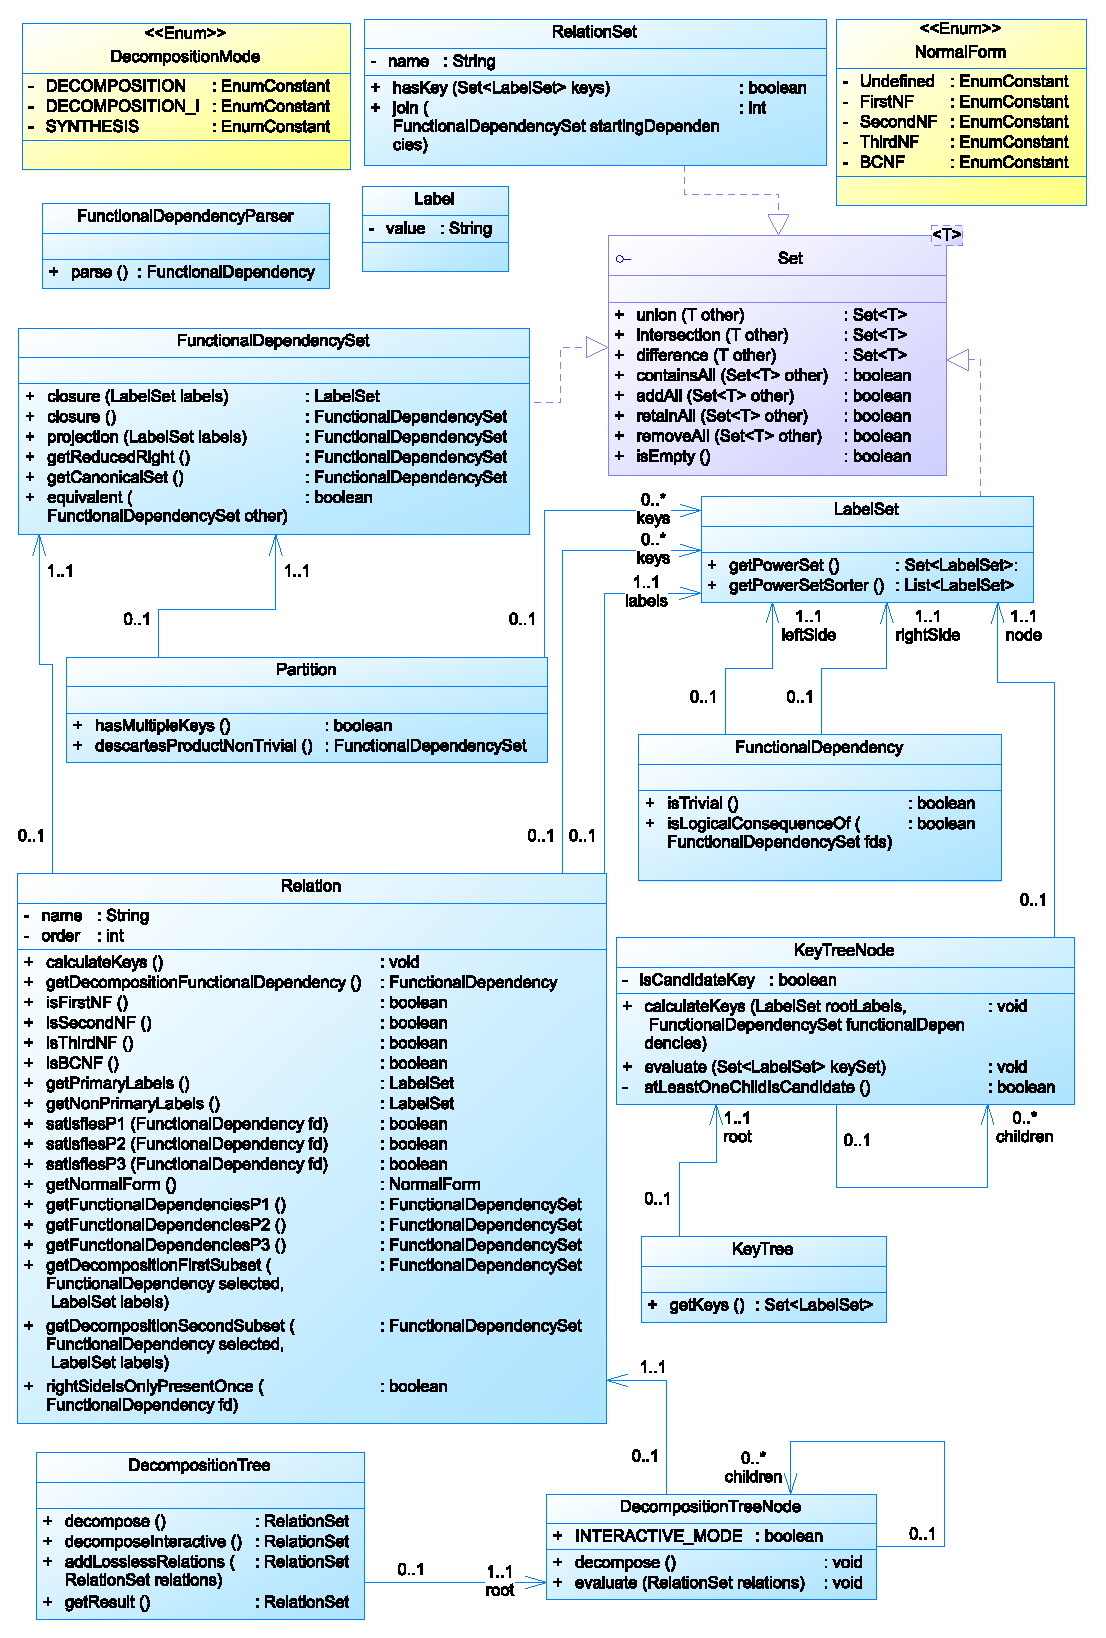
\includegraphics[width=1\textwidth]{ClassDiagram_1}
    \caption{\textit{RelNorm} osztálydiagram}
    \label{fig:class}
\end{figure}
 
\section{Alapvető algoritmusok/kódrészletek}

Ebben a részben az előző fejezetben leírt alapvető relációs fogalmak és műveletek algoritmusainak a megvalósítása kerül bemutatásra.

Az attribútumhalmaz lezártjának a definícióját (~\ref{eq:closure} képlet) a függőséghalmaz \lstinline{closure} metódusával tudjuk kiszámolni:

\linespread{1}
\begin{lstlisting}[language=Java]
public LabelSet closure(LabelSet labels) {
	LabelSet result = new LabelSet(labels);
	LabelSet lastResult;
	do {
		lastResult = new LabelSet(result);

		this.items.forEach(fd -> {
			if(result.containsAll(fd.getLeftSide())) {
				result.addAll(fd.getRightSide());
			}
		});
	} while(!lastResult.equals(result));
	return result;
}
\end{lstlisting}

A függőséghalmaz projekcióját (~\ref{eq:projection} képlet) a függőséghalmaz \lstinline{projection} metódusával tudjuk kiszámolni:

\linespread{1}
\begin{lstlisting}[language=Java]
public FunctionalDependencySet projection(LabelSet labels) {
	FunctionalDependencySet projection = new FunctionalDependencySet();
	for(LabelSet subset: labels.getPowerSet()) {
		LabelSet closure = this.closure(subset);
		closure.retainAll(labels);
		closure.removeAll(subset);
		if(!closure.isEmpty()) {
			FunctionalDependency fd = 
			    new FunctionalDependency(subset, closure);
			projection.add(fd);
		}
	}
	return projection;
}
\end{lstlisting}

A fenti kódrészletben szerepel egy \lstinline{getPowerSet} nevezetű metódus, amely egy adott attribútumhalmaz összes részhalmazának a halmazát számolja ki \parencite{baeldung2020}.

Az igaz következmény, azaz egy függőséghalmazhoz viszonyított függőség logikai következényének a definícóját (~\ref{eq:setclosure} képlet) az attribútumhalmaz \lstinline{isLogicalConsequenceOf} metódusával lehet kiszámolni.

\linespread{1}
\begin{lstlisting}[float,floatplacement=H,language=Java]
public boolean isLogicalConsequenceOf(FunctionalDependencySet dependencies) {
	LabelSet closure = dependencies.closure(leftSide);
	return closure.containsAll(rightSide);
}
\end{lstlisting}

Két függőséghalmaz egybevágóságát (~\ref{eq:equiv} képlet) a függőséghalmaz equivalent metódusa számolja ki.

\linespread{1}
\begin{lstlisting}[float,floatplacement=H,language=Java]
public boolean equivalent(FunctionalDependencySet other) {
	return 
		this.stream().allMatch(fd -> fd.isLogicalConsequenceOf(other)) &&
		other.stream().allMatch(fd -> fd.isLogicalConsequenceOf(this));
}
\end{lstlisting}

A relációs sémák kulcshalmazához az előző fejezetben leírt algoritmust (~\ref{eq:reductionop} képlet) használjuk. A megvalósításhoz elengedhetetlen egy ún. \textit{kulcsfa} \index{kulcsfa (ang. \textit{key tree})} használata. Ez a kulcsfa olyan csomópontokból áll össze, melyek tartalmaznak egy atribútumhalmazt, információt a kulcsjelölti státuszukról valamint egy kollekciót a gyermekeiről. A gyermek csomópont pontosan egy attribútummal kevesebbet tartalmaz a szülőtől. Ha egy megadott attribútumhalmaz $U=\{A,B,C,D\}$ és függőséghalmaz $F=\{AC \to B,BC \to D,A \to B,B \to A\}$ kulcsait szeretnénk megkapni ($K=\{AC,BC\}$), akkor a(z) ~\ref{fig:keytree} ábra mutatja be ennek a példának a kulcsfáját.

\begin{figure}
    \centering
    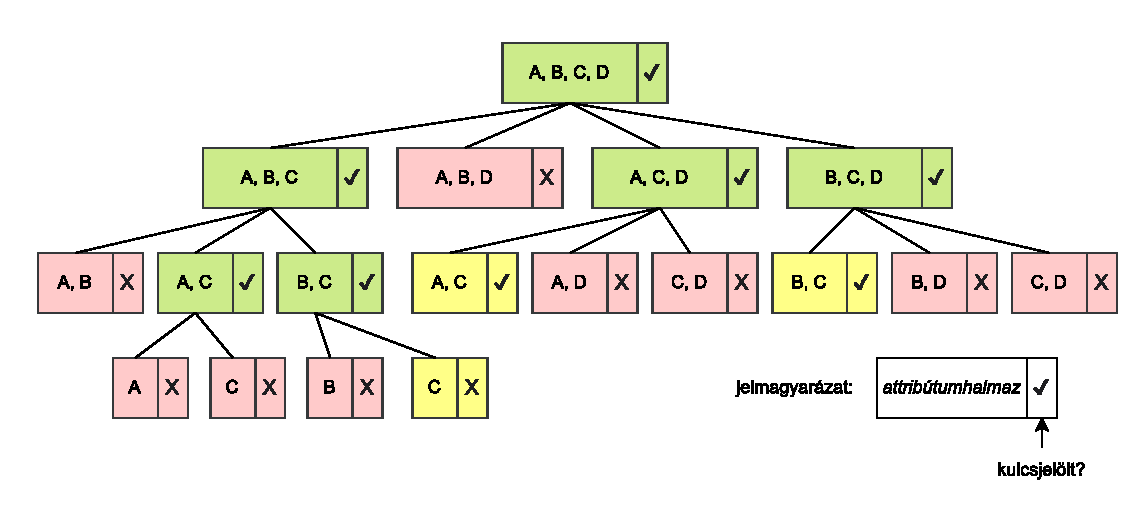
\includegraphics[width=1\textwidth]{keytree}
    \caption{Kulcsfa}
    \label{fig:keytree}
\end{figure}

A zölddel jelölt csomópontokat további rekurzív számításnak vetjük alá mindaddig, amíg egy csomópont kulcsjelölti státusza meg nem szűnik (piros) vagy már az adott csomópont attribútumhalmazát bejártuk (sárga). A kulcsfa kiértékelésénél azokat a zöld csomópontokat tekintjük kulcsnak, amelyek kulcsjelöltek, de egyik gyermekük sem kulcsjelölt.

\section{Normálformák megvalósítása}

Az első normálforma, azaz az \textit{1NF} előzetes megegyezés szerint mindig teljesítve lesz, mivel a normalizációs algoritmusok nem tudják megállapítani egyes attribútumok struktúráját.

\linespread{1}
\begin{lstlisting}[language=Java]
public boolean isFirstNF() {
	return true;
}
\end{lstlisting}

Az első normálformán túl szükségünk van további kisegítő metódusokra. Ilyen metódusok a primáris és szekundáris attribútumhalmazt kiszámoló metódusok. A primáris attribútumok a \lstinline{getPrimaryLabels} metódussal kaphatóak meg.

\linespread{1}
\begin{lstlisting}[language=Java]
private LabelSet getPrimaryLabels() {
	LabelSet primaryLabels = new LabelSet();
	keys.forEach(primaryLabels::addAll);
	return primaryLabels;
}
\end{lstlisting}

A szekundáris attribútumok a \lstinline{getNonPrimaryLabels} metódussal kaphatóak meg.

\linespread{1}
\begin{lstlisting}[language=Java]
private LabelSet getNonPrimaryLabels() {
	LabelSet allLabels = new LabelSet(labels);
	allLabels.removeAll(getPrimaryLabels());
	return allLabels;
}
\end{lstlisting}

A reláció \lstinline{isSecondNF} metódusával kapjuk meg azt az információt, hogy egy adott reláció teljesíti-e a \textit{2NF} normálformát annak definíciója szerint (~\ref{eq:2nf} képlet).

\linespread{1}
\begin{lstlisting}[language=Java]
public boolean isSecondNF() {
	LabelSet nonPrimaryLabels = getNonPrimaryLabels();
	if(nonPrimaryLabels.isEmpty()) {
		return true;
	}

	return functionalDependencies.stream().allMatch(fd -> {
		if(nonPrimaryLabels.containsAll(fd.getRightSide())) {
			return getKeys().stream().allMatch(key -> 
				fd.getLeftSide().containsAll(key) || 
				fd.getLeftSide().stream().noneMatch(key::contains));
		} else {
			return true;
		}
	});
}
\end{lstlisting}

A \textit{3NF} normálformának az alternatív definíciója alapján (~\ref{eq:3nfalt} képlet) készült el a relációs séma \lstinline{isThirdNF} metódusa.

\linespread{1}
\begin{lstlisting}[language=Java]
public boolean isThirdNF() {
	LabelSet nonPrimaryLabels = getNonPrimaryLabels();
	if(nonPrimaryLabels.isEmpty()) {
		return true;
	}

	return functionalDependencies.stream().allMatch(fd -> {
		if(nonPrimaryLabels.containsAll(fd.getRightSide())) {
			return getKeys().stream().anyMatch(key -> 
				fd.getLeftSide().containsAll(key));
		} else {
			return true;
		}
	});
}
\end{lstlisting}

A \textit{BCNF} normálforma definíciója (~\ref{eq:bcnf} képlet) alapján létrejött \lstinline{isBCNF} metódussal számítható ki, hogy egy relációs séma teljesíti-e a \textit{BCNF} normálformát.

\linespread{1}
\begin{lstlisting}[language=Java]
public boolean isBCNF() {
	return functionalDependencies.stream()
		.filter(fd ->!fd.isTrivial())
		.allMatch(fd -> getKeys().stream().
			anyMatch(key -> fd.getLeftSide().containsAll(key)));
}
\end{lstlisting}

Tekintettel a ~\ref{eq:nf} képletekre, egy bizonyos relációs séma normálformájának a megállapítását a \lstinline{getNormalForm} metódussal valósítottuk meg.

\linespread{1}
\begin{lstlisting}[language=Java]
public NormalForm getNormalForm() {
	return isBCNF() ? NormalForm.BCNF :
     			isThirdNF() ? NormalForm.ThirdNF :
				isSecondNF() ? NormalForm.SecondNF :
					isFirstNF() ? NormalForm.FirstNF : 
						NormalForm.Undefined;
}
\end{lstlisting}

\section{Szintézis algoritmusának a megvalósítása}

A szintézis algoritmusának számítógépes megvalósítását a(z) ~\ref{fig:synseq} ábra tükrözi. Felhasználói beavatkozás, ami befolyásolná az algoritmus kimenetelét, nem történik a lefuttatás alatt.

\begin{figure}
    \centering
    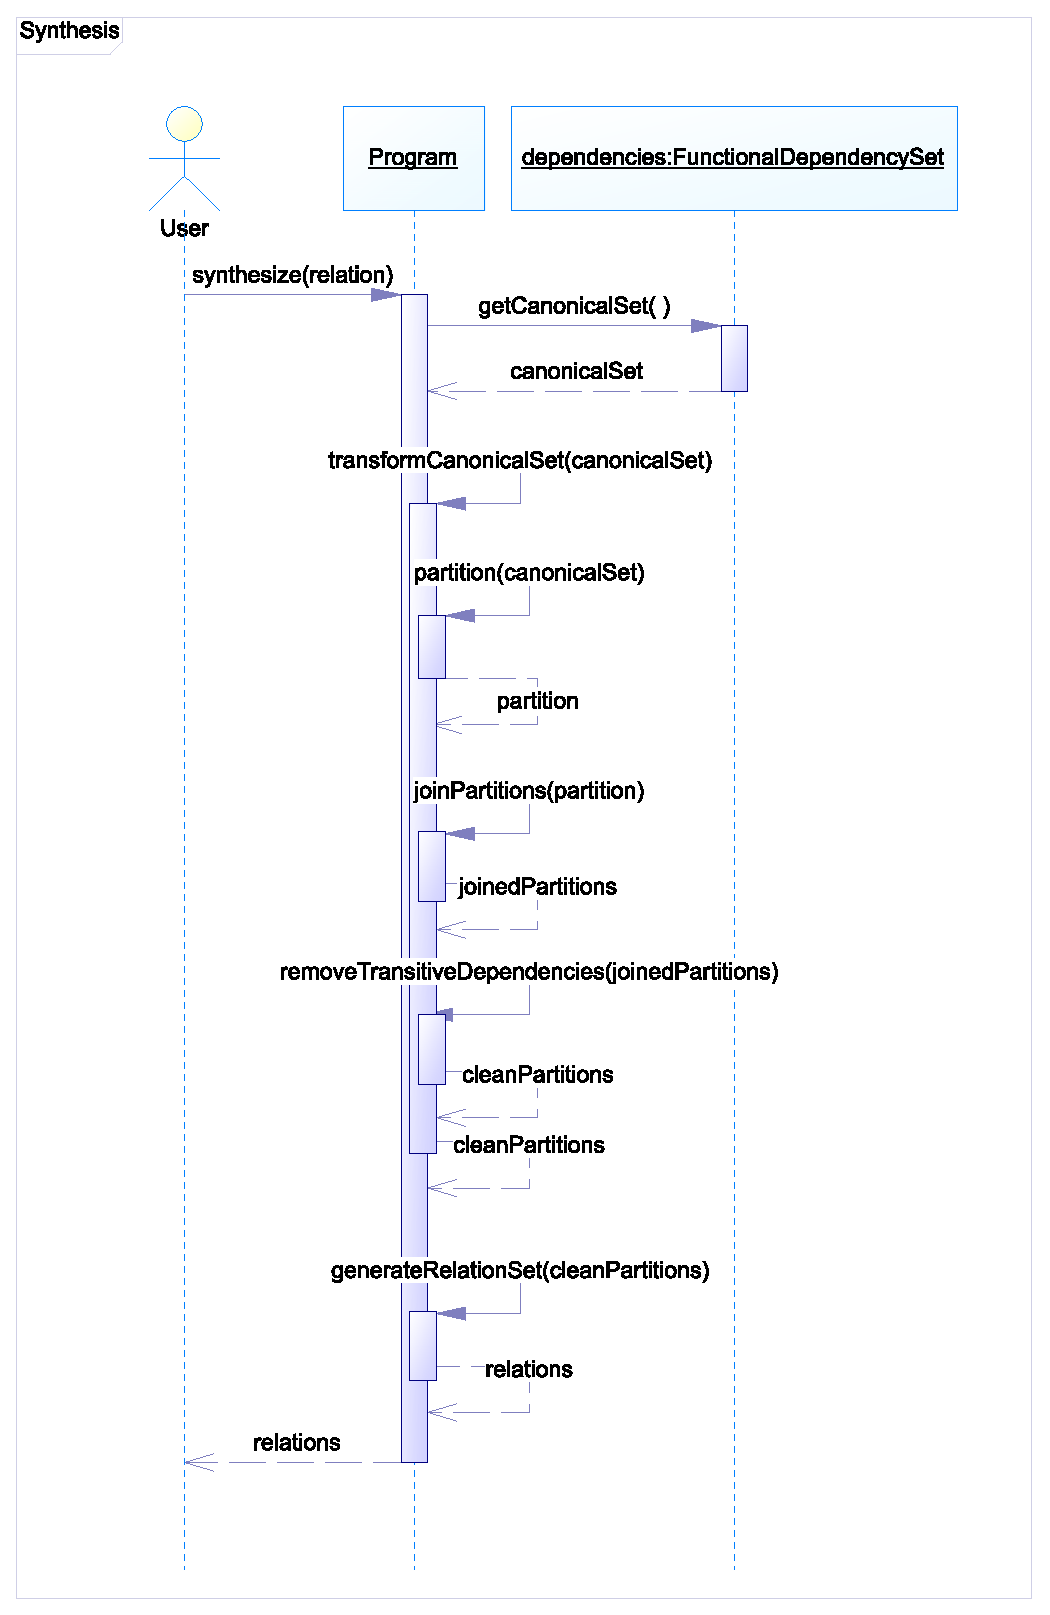
\includegraphics[width=0.95\textwidth]{Synthesis}
    \caption{A szintézis szekvenciadiagramja}
    \label{fig:synseq}
\end{figure}

A szintézis algoritmusa alapján a legfontosabb lépés a minimális függéshalmaz kiszámolása. Ezt három lépésből tudjuk megtenni: A minimális függéshalmazban a függőségek jobboldali attribútumhalmazában csak egyetlen attribútum található (~\ref{eq:syn1-2} képlet), a függőségek teljes függőségek (~\ref{eq:syn1-3} képlet), valamint nincs olyan függőség, amelyik elhagyható (~\ref{eq:syn1-4} képlet).

\begin{enumerate}

    \item A jobboldali függőségek egy atribútummá való redukálása:
    
\linespread{1}
\begin{lstlisting}[language=Java]
FunctionalDependencySet reduced = new FunctionalDependencySet();
items.forEach(
	fd -> fd.getRightSide().forEach(
		label -> reduced.add(
			new FunctionalDependency(fd.getLeftSide(), label))
	)
);
\end{lstlisting}

    \item A részleges függőségek teljes függésé való átalakítása
    
\linespread{1}
\begin{lstlisting}[language=Java]
FunctionalDependencySet reducedS = new FunctionalDependencySet(canonicalSet);
reduced.forEach(
	fd -> fd.getLeftSide().getPowerSetSorted().stream()
	.filter(subset -> !subset.isEmpty() && !subset.equals(fd.getLeftSide()))
	.map(subset -> new FunctionalDependency(subset, fd.getRightSide()))
	.filter(partial -> partial.isLogicalConsequenceOf(reducedS))
	.limit(1)
	.forEach(partial -> {
		reducedS.add(partial);
		reducedS.remove(fd);
	})
);
\end{lstlisting}

    \item Elhagyható függőségek törlése
    
\linespread{1}
\begin{lstlisting}[language=Java]
FunctionalDependencySet setToRemove = new FunctionalDependencySet();
reducedS.stream()
	.filter(fd ->
		fd.isLogicalConsequenceOf(
			reducedS.difference(fd).difference(setToRemove)))
	.forEach(setToRemove::add);
reducedCanonicalSet.removeAll(setToRemove);
\end{lstlisting}
\end{enumerate}

A partíciók kialakításához először egy \lstinline{HashMap} kollekcióba rendeztük a függőségeket, a baloldali attribútumhalmazaitól függően. Ezután ezeknek a baloldali attribútumhalmazoknak kiszámoltuk a zártját, és amennyiben azok megegyeztek, összevontuk ezeket a partíciókat. Ezek az algoritmusok viszonylag egyszerűek, ezért nem kerülnek bemutatásra ebben a dolgozatban.

Ezután következik az összevonás által keletkezett potenciálisan tranzitív függőségek eltávolítása a partíciókból. Ennek kiszámolása érdekében a következőképpen létrehozzuk a $J$ függőséghalmazt (~\ref{eq:syn2-6} képlet).

\linespread{1}
\begin{lstlisting}[language=Java]
FunctionalDependencySet jay = new FunctionalDependencySet();
for(Partition partition: partitions) {
	FunctionalDependencySet desc = partition.descartesProductNonTrivial();
	FunctionalDependencySet descReduced = descartes.getReducedRight();
	jay.addAll(descReduced);
	partition.removeAll(descReduced);
}
\end{lstlisting}

A \lstinline{descartesProductNonTrivial} metódus kiszámolja az összevont partícióknak az ún. permutációs (nem triviális) függőséghalmazát (~\ref{eq:syn2-7} képlet). Azaz, ha $A$, $B$ és $C$ kulccsal rendelkező partíciókat vontunk össze, akkor ez a metódus eredményként $A \to B$, $B \to A$, $A \to C$, $C \to A$, $B \to C$ és $C \to B$ függőségeket eredményezi. Majd ezeken a függőségeken jobb oldali egyszerűsítést végzünk annak érdekében, hogy a jobboldali attribútumhalmaz csak egy attribútumot tartalmazzon.

A tranzitív függőségek eltávolításához befejező lépésként megalkotjuk az $M$ függőséghalmazt (~\ref{eq:syn2-8} képlet).

\linespread{1}
\begin{lstlisting}[language=Java]
FunctionalDependencySet em = new FunctionalDependencySet();
em.addAll(jay);
partitions.forEach(p -> em.addAll(p.getValues()));

partitions.forEach(partition -> {
	FunctionalDependencySet functionalDependenciesCopy =
		new FunctionalDependencySet(partition.getValues());
		functionalDependenciesCopy.forEach(fd -> {
    public ChannelService(ChannelRepository repository, OrganizationService organizationService, FilesystemUtil fsUtil) {
        this.repository = repository;
        this.organizationService = organizationService;
        this.fsUtil = fsUtil;
    }
			if(fd.isLogicalConsequenceOf(em.difference(fd))) {
				partition.remove(fd);  // fd is transitive dependency
			}
		});
});

partitions.forEach(partition -> partition.addAll(jay));
\end{lstlisting}

A relációs séma halmaza a szintézis algoritmusa alapján megfelel a létrejött partícióknak, amit így alkotunk meg:

\linespread{1}
\begin{lstlisting}[language=Java]
RelationSet relations = new RelationSet("S");
int n = 1;
for(Partition partition : partitions) {
	LabelSet labels = partition.getLabels();
	Relation relation = 
		new Relation("S", n++, labels, partition.getValues());
	relations.add(relation);
}
\end{lstlisting}

A veszteségmentes sémafelbontást érdekében a kezdetleges relációs séma egyik kulcsát tartalmazó relációs sémát hozunk létre, amennyiben olyan relációs séma nem képezi az eddig létrejötteket:

\linespread{1}
\begin{lstlisting}[language=Java]
if(!relations.hasKey(initialRelation.getKeys())) {
	Relation lossless = 
		new Relation("S", n, 
			initialRelation.getKeys().stream().findAny().get(),
			new FunctionalDependencySet());
	relations.add(lossless);
}
\end{lstlisting}

\section{Dekompozíció algoritmusának a megvalósítása}

A dekompozíció első lépése a megfelelő függőség kiválasztása. Ezt a függőséget háromféle kritérium alapján tudjuk kiválasztani. A következő metódusok azt vizsgálják, hogy egy adott függőség megfelel-e a P1 (~\ref{eq:p1}), P2 (~\ref{eq:p2}) illetve a P3 (~\ref{eq:p3}) kritériumnak. 

\linespread{1}
\begin{lstlisting}[language=Java]
public boolean satisfiesP1(FunctionalDependency fd) {
	return !fd.isTrivial() &&
		keys.stream().noneMatch(k -> fd.getLeftSide().containsAll(k)) && 
		functionalDependencies.equivalent(
			functionalDependencies.projection(fd.getLeftSide()
				.union(labels.difference(fd.getRightSide())))
		.union(functionalDependencies.projection(fd.getLeftSide()
				.union(fd.getRightSide()))));
}
\end{lstlisting}

\linespread{1}
\begin{lstlisting}[language=Java]
public boolean satisfiesP2(FunctionalDependency fd) {
	return !fd.isTrivial() &&
		!fd.getLeftSide().union(fd.getRightSide()).containsAll(labels) &&
		functionalDependencies.equivalent(
			functionalDependencies.projection(fd.getLeftSide()
				.union(labels.difference(fd.getRightSide())))
			.union(functionalDependencies.projection(fd.getLeftSide()
				.union(fd.getRightSide()))));
}
\end{lstlisting}

\linespread{1}
\begin{lstlisting}[language=Java]
public boolean satisfiesP3(FunctionalDependency fd) {
	return !fd.isTrivial() && keys.stream().noneMatch(k ->
		fd.getLeftSide().containsAll(k));
}
\end{lstlisting}

A szintézis algoritmussal ellentétben, a dekompozíció algoritmusánál a felhasználó is beleszólhat az algoritmus lefolyásába. Ezt oly módon teszi, hogy a felkínált függőségekből (melyek lehetőleg minél nagyobb kritériumi szintet teljesítenek) választ egyet. A(z) ~\ref{fig:dectree} ábra bemutatja, hogy minderre a \lstinline{decompose} metódus elején kerül sor – a \lstinline{user selects functional dependency} üzenettel. Az algoritmus interaktív mivolta úgy valósul meg, hogy a program a standard kimenetre nyomtatja a választható függőségeket, a felhasználó pedig a billentyűzet segítségével kiválasztja a neki megfelelő függőséget. Az algoritmus automatikus változata ezt a választás lehetőségét átugorja, és találomra választ egy függőséget a felkínáltak közül.

Mivel a dekompozíció lépéseiben az algoritmus az aktuális relációs sémát két relációs sémára válassza szét (~\ref{eq:r1r2} képlet), innen ered az ötlet, hogy a dekompozíció megvalósításához elég létrehozni egy ún. dekompozíciós fát. Ennek a fának a csomópontjai relációs sémák lesznek, a levelei pedig a dekompozíció eredményeként létrejött relációs sémahalmazt alkotják.

\begin{figure}
    \centering
    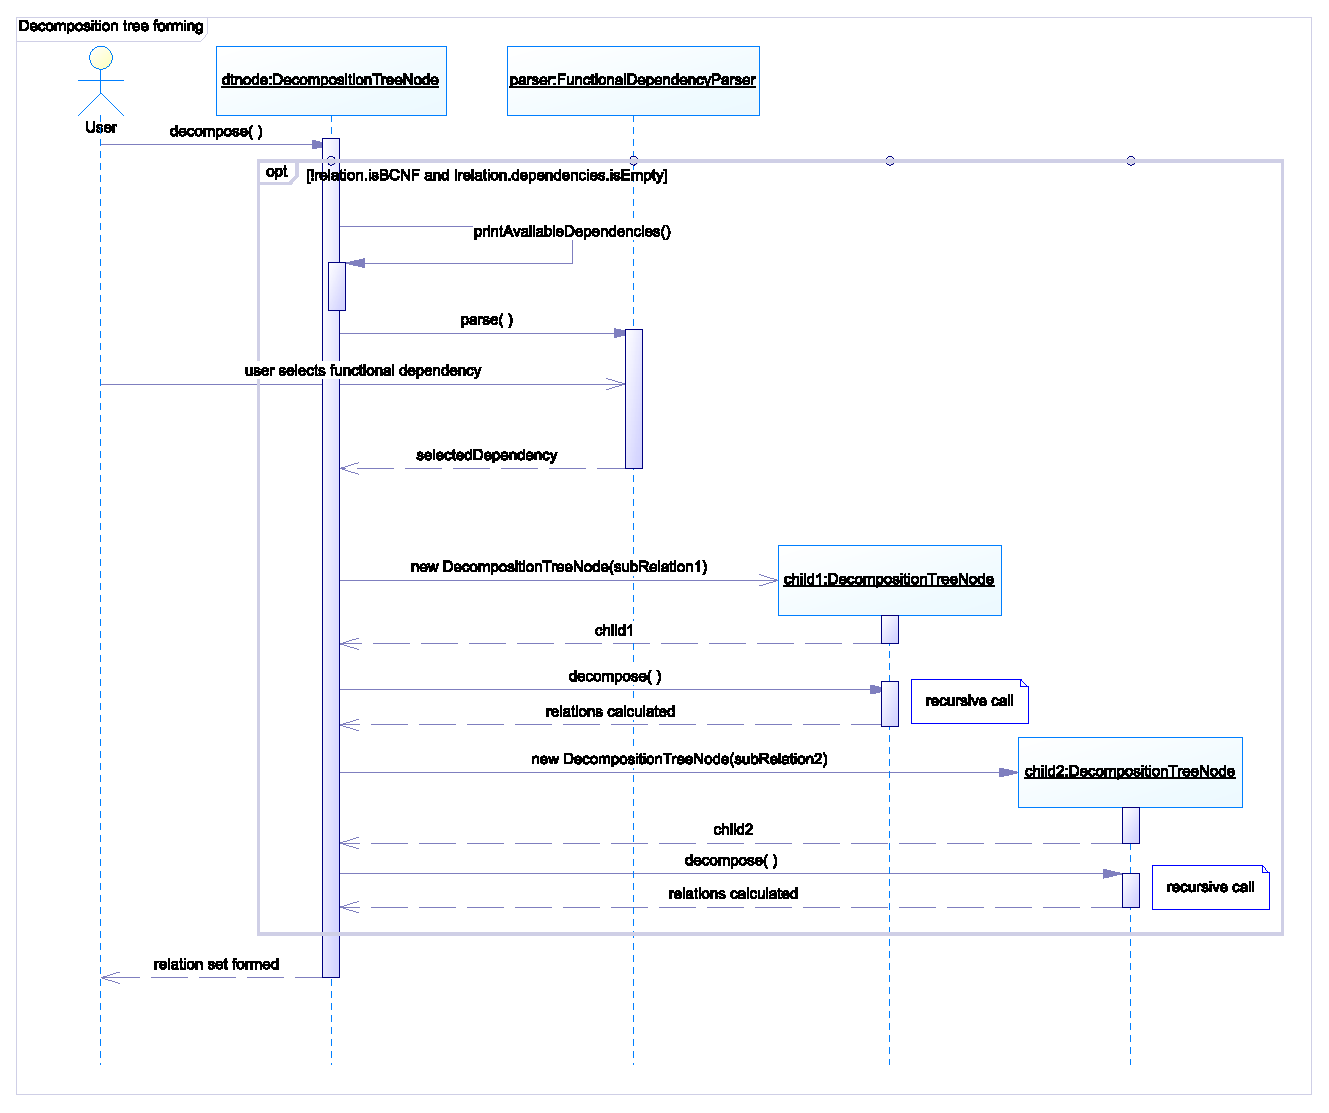
\includegraphics[width=1\textwidth]{Decomposition_tree_forming}
    \caption{A dekompozíciós fa formálásának a szekvenciadiagramja}
    \label{fig:dectree}
\end{figure}

A dekompozíciós fa létrejöttéhez a \lstinline{decompose} metódus rekurzív előhívása szükséges a relációs séma dekomponált gyermekcsomópontjain. Ez a folyamat addig folytatódik, amíg nem kapunk olyan relációs sémákat, amelyek teljesítik a \textit{BCNF} normálformát.

Miután létrehoztuk az ún. dekompozíciós fát, ki kell értékelni azt. Ezt szintén rekurzív módszerekkel oldottuk meg (~\ref{fig:decomposition} ábra). A fa leveleinek a begyűjtése után ki kell vizsgálni, hogy az azonos kulcsokkal rendelkező relációs sémákat összevonjuk, majd leellenőrizzük a veszteségmentes sémafelbontás feltételeit. Ezt hasonlóképp végezzük el, mint a szintézis algoritmusa során. 

\begin{figure}
    \centering
    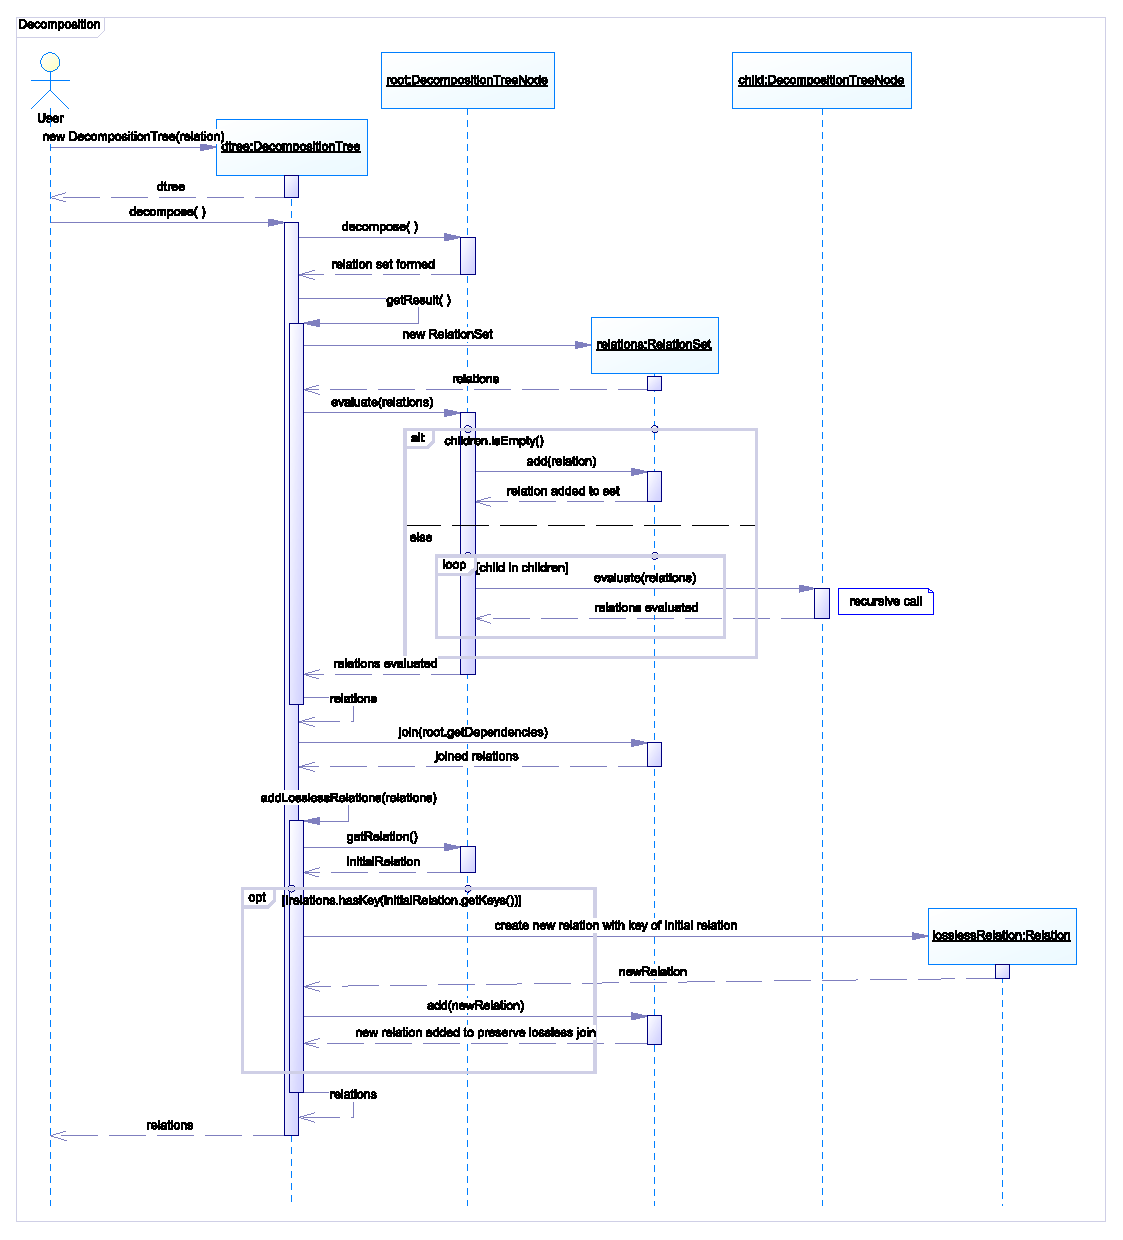
\includegraphics[width=1\textwidth]{Decomposition}
    \caption{A dekompozíciós fa kiértékelésének a szekvenciadiagramja}
    \label{fig:decomposition}
\end{figure}

\section{Egyéb magvalósítási részletek}

A dolgozatban felvázolt célkitűzések között szerepel az a követelmény, hogy a feladatsorok könnyen megadhatóak és cserélhetőek legyenek. Ennek a követelménynek tettünk eleget, hogy szöveges úton engedélyeztük a program bemeneti feladatsorát. A felhasználó egy \textit{JSON} típusú fájlként tudja megadni a feladatsorát, majd lefuttatáskor a megfelelő fájlt tudja bemenetként megadni.

Példaként szolgálva, ha egy $N$ nevezetű relációnak az attribútumhalmaza $\{A,B,C,D,E\}$, függőséghalmaza pedig $\{AB \to CE, C \to D\}$, akkor a bemeneti feladatsor fájlja a következőképp néz ki:

\linespread{1}
\begin{lstlisting}
{
  "name": "N",
  "labels": ["A", "B", "C", "D", "E"],
  "functionalDependencies": [
    {"left": ["A", "B"], "right": ["C", "E"]},
    {"left": ["C"], "right": ["D"]}
  ]
}
\end{lstlisting}

A forráskód felépítéséhez és becsomagolásához a \textit{Maven} eszköz \lstinline{package} parancsa szükséges:

\linespread{1}
\begin{lstlisting}[language=sh]
mvn package
\end{lstlisting}

A sikeres csomagolás után a build mappában fog szerepelni a \textit{JAR} csomag, melyet a következőképp tudunk lefuttatni:

\linespread{1}
\begin{lstlisting}[language=sh]
java -jar rel-norm-1.0-SNAPSHOT.jar <task> <method>
\end{lstlisting}

A \lstinline{<task>} megjelölés helyett a feladatsor fájljának az útvonalát kell megadni, a \lstinline{<method>} megjelölés helyett meg egyikét a következőnek:

\begin{itemize}
    \item \lstinline{DECOMPOSITION} -- a dekompozíció algoritmus lefuttatásához,
	\item \lstinline{DECOMPOSITION_I} -– a dekompozíció interaktív algoritmusának lefuttatásához és
	\item \lstinline{SYNTHESIS} -- a szintézis algoritmusának a lefuttatásához.
\end{itemize}
	
\section{Szoftvertesztek megvalósítása}

A \textit{Java} programnyelvnek rendeltetésszerű tesztelési munkakeretét használtuk a dolgozatban. A munkakeret neve \textit{JUnit}, ami unit-tesztek írását és lefuttatását teszi lehetővé. A dolgozat ~\ref{ch:elmelet}. fejezetében felsorolt relációs műveletek és algoritmusok mindegyike szerepel a teszt esetekben. A tesztek érvényességét feladatgyűjteményből \parencite{kordic2018} származtatott feladatok és megoldásaik szavatolják. A tesztek elindításához a következő parancsot kell végrehajtani:

\linespread{1}
\begin{lstlisting}[language=sh]
mvn test
\end{lstlisting}

A kód lefedettség kiszámolása érdekében külső szoftverelemző eszközt használunk. A \textit{SonarCloud} online kódbázis elemző szoftver, amivel git alapú kódbázisokat tudunk megfigyelni. A \textit{SonarCloud} képes jelenteni programhibákat, biztonsági réseket, nem tiszta kód jellemzőit, kód többszöröződést stb. Mindezek mellett még kód lefedettségi szintet is mér, habár ezt külső tesztjelentésből állítja össze. Ahhoz, hogy a \textit{SonarCloud} külső tesztjelentéseket tudjon olvasni, integrálni kell a \textit{JaCoCo} bővítményt a \textit{Maven} projektbe. Ez a bővítmény jelentéseket készít a lefuttatott tesztekről.

\chapter{Eredmények}

Az előző fejezetben leírt algoritmusok megvalósításának a helyességét úgy tudjuk leellenőrizni, ha szoftvertesztekkel támasztjuk alá a működésüket. Ezeknek a teszteknek az eredményei a ~\ref{tab:teszt} táblázatban szerepelnek. Valamennyi algoritmus metódusához rendeltünk legalább 2 tesztet, hogy megbizonyosodjunk arról, hogy a tesztek nem csak véletlenszerűen sikerültek. A teszt eseteket feladatlapból \parencite{kordic2018} szerzett feladatokra alapoztuk, melyeknek ismertek az eredményei. Ezek az ismert eredmények kerültek összehasonlításra az algoritmus által kapott eredményekkel. Amennyiben az eredmények nem egyeztek meg, azokat sikertelen teszteknek vettük; ha hiba keletkezett tesztelés során, azok a hibák száma oszlopban vannak feltüntetve. Ha bármiféle okból kifolyólag nem lehetett lefuttatni a tesztet, az az átugrott tesztek számát növelte. A tesztek mellett feltüntetett eltelt idő az egyes tesztcsoportok lefutásának az idejét jegyzi.

\begin{table}
    \centering
    \begin{tabular}{|b{4cm}|b{1.5cm}|b{1.8cm}|b{1.5cm}|b{1.5cm}|b{1.5cm}|}
    \hline
    Teszt neve & Tesztek száma & Sikertelen tesztek száma & Hibák száma & Átugrott tesztek száma & Eltelt idő [ms] \\
    \hline \hline
    LogicalConsequence & 5 & 0 & 0 & 0 & 2 \\ \hline
    AttributeSetClosure & 6 & 0 & 0 & 0 & 3 \\ \hline
    Equivalence & 2 & 0 & 0 & 0 & 1 \\ \hline
    Projection & 3 & 0 & 0 & 0 & 1 \\ \hline
    Keys & 3 & 0 & 0 & 0 & 5 \\ \hline
    RelationParser & 2 & 0 & 0 & 0 & 66 \\ \hline
    2NF & 5 & 0 & 0 & 0 & 25 \\ \hline
    3NF & 2 & 0 & 0 & 0 & 1 \\ \hline
    NormalForm & 4 & 0 & 0 & 0 & 5 \\ \hline
    CanonicalSet & 4 & 0 & 0 & 0 & 39 \\ \hline
    \textbf{Decomposition} & 4 & 0 & 0 & 0 & 97 \\ \hline
    \textbf{Synthesis} & 6 & 0 & 0 & 0 & 108 \\ \hline
    \hline
    TOTAL & 46 & 0 & 0 & 0 & 353 \\ \hline
    \end{tabular}
    \caption{Szoftvertesztelés eredménye}
    \label{tab:teszt}
\end{table}

A \textit{SonarCloud} szoftverelemző eszköz jelentésének egy részét a ~\ref{tab:sonar} táblázat jeleníti meg. Ez a jelentés magában foglal különböző statisztikai adatokat a teljes kódbázisról, amit a \textit{SonarCloud} bizonyos belső algoritmusok és kritériumok alapján számol.

\begin{table}
    \centering
    \begin{tabular}{|l|r|}
    \hline
    Jellemző & Érték \\ \hline
    \hline
    Összes kódsor & 1161 \\ \hline
    Osztályok száma & 21 \\ \hline
    Kommentek aránya & 1.4 \\ \hline
    Code Smell & 30 \\ \hline
    Biztonsági rések & 0 \\ \hline
    Kódtöbbszöröződés & 0\% \\ \hline
    Hibák & 0 \\ \hline
    Teszt lefedettség & 76.5\% \\ \hline
    \end{tabular}
    \caption{SonarCloud elemzésének az eredményei}
    \label{tab:sonar}
\end{table}


\chapter{Tárgyalás}

Az előző fejezet szoftvertesztelési eredményei alapján kijelenthető, hogy a \textit{RelNorm} eszköz sikeresen el tudja végezni a relációs adatbázisok normalizációját a szintézis és a dekompozíció algoritmusát felhasználva. Ezek az algoritmusok relatív több időt igényelnek, mint a kisebb összetettségű algoritmusok, és ez a teszteredményeken is meglátszik. A \lstinline{RelationParser} teszt esetek ugornak ki a sorból a hosszabb futtatási idővel. Ezekben az esetekben fájl beolvasása történik, ezzel magyarázható a hosszabb futtatási idő. A dekompozíció algoritmusánál nem sikerült tesztelni az interaktív függőség megadás módszerét, ezért az interaktív módszer azon pontján, ahol felhasználói bemenet szükséges, automatikusan kiválasztja a program a felkínált függőségek egyikét.

A \textit{SonarCloud} jelentése nem okozott kiugró értékeket. Megemlíthető azonban a \textit{Code Smell} jellemző, ami a nem tiszta kód jellemzőit számlálja. Ez az érték 30 lett, ami egy relatív magas szám. Ennek a 30 észrevételnek túlnyomó többsége a felhasználóval való interakciót jelezte, pontosabban a standard bemenet és kimenet használatát kifogásolta. Mivel a \textit{RelNorm} egy konzol applikáció, ezért egyelőre nincs más módja a felhasználói bemenet megváltoztatására.

A teszt lefedettség 76.5\% lett, ami szintén egy jó eredmény. Betekintve az elemzés részleteibe, a lefedettség azért nem lett nagyobb, mert nem került tesztelésre valamennyi konstruktőr, get/set metódus, beépített metódus, valamint a standard bemenettel és kimenettel foglalkozó metódusok sem.

\chapter{Összefoglalás}

Ebben a dolgozatban bemutatásra került a \textit{RelNorm} nevezetű szoftver, amely relációs adatbázisok normalizálásának a problémáját próbálja megoldani. A \textit{RelNorm} eszközt elsősorban oktatásban ajánlott alkalmazni, normalizálási feladatsorok összeállításánál és a megoldott feladatok leellenőrzésénél. A dolgozat bemutatja a hasonló normalizálási szoftvereket, majd a legalapvetőbb relációs fogalmakra és algoritmusokra tér rá. A \textit{RelNorm} fejlesztési fázisai a(z) \ref{ch:gyakorlat}. fejezetben kerültek be a dolgozatba, ahol kódrészletekkel valamint osztály- és szekvenciadiagramokkal prezentáltuk a szoftver megvalósítását. A \textit{RelNorm} szoftvertesztelésnek vetettük alá, ezek eredményei és kiértékelése a dolgozat utolsó fejezetében történt.

A bemutatott eredmények és azok elemzésének fényében következtethető, hogy a \textit{RelNorm} teljesítette a dolgozatban elé támasztott követelményeket. A gyakorlatban a 2021--2022-es tanévben már helytállt szoftver kielégítette azokat az igényeket, melyeket tanársegédi feladatokként szántunk a szoftverhez.

Jövőbeli terveink között szerepel egy grafikus felhasználói felület kifejlesztése, ami akár web applikációs formát is ölthet: így a \textit{RelNorm} szélesebb rétegekhez is eljuthat. Amennyiben igény van rá, akkor további funkciókkal is bővíthető a program, ami egy tanulási keretet is adhat a hallgatóknak.
\printbibliography[heading=bibintoc,title={Irodalomjegyzék}]

\printindex

\end{document}
